\documentclass[a4paper,12pt]{extarticle}
\usepackage[utf8x]{inputenc}
\usepackage[T1,T2A]{fontenc}
\usepackage[russian]{babel}
\usepackage{hyperref}
\usepackage{indentfirst}
\usepackage{listings}
\usepackage{color}
\usepackage{here}
\usepackage{array}
\usepackage{multirow}
\usepackage{graphicx}

\usepackage{caption}
\renewcommand{\lstlistingname}{Программа} % заголовок листингов кода

\bibliographystyle{ugost2008ls}
\linespread{1.3}

\usepackage{listings}
\lstset{ %
extendedchars=\true,
keepspaces=true,
language=C,						% choose the language of the code
basicstyle=\footnotesize,		% the size of the fonts that are used for the code
numbers=left,					% where to put the line-numbers
numberstyle=\footnotesize,		% the size of the fonts that are used for the line-numbers
stepnumber=1,					% the step between two line-numbers. If it is 1 each line will be numbered
numbersep=5pt,					% how far the line-numbers are from the code
backgroundcolor=\color{white},	% choose the background color. You must add \usepackage{color}
showspaces=false				% show spaces adding particular underscores
showstringspaces=false,			% underline spaces within strings
showtabs=false,					% show tabs within strings adding particular underscores
frame=single,           		% adds a frame around the code
tabsize=2,						% sets default tabsize to 2 spaces
captionpos=t,					% sets the caption-position to top
breaklines=true,				% sets automatic line breaking
breakatwhitespace=false,		% sets if automatic breaks should only happen at whitespace
escapeinside={\%*}{*)},			% if you want to add a comment within your code
postbreak=\raisebox{0ex}[0ex][0ex]{\ensuremath{\color{red}\hookrightarrow\space}},
inputpath=listings,                     % директория с листингами
}

\usepackage[left=2cm,right=2cm,
top=2cm,bottom=2cm,bindingoffset=0cm]{geometry}

%% Нумерация картинок по секциям
\usepackage{chngcntr}
\counterwithin{figure}{section}
\counterwithin{table}{section}

%%Точки нумерации заголовков
\usepackage{titlesec}
\titlelabel{\thetitle.\quad}
\usepackage[dotinlabels]{titletoc}

%% Оформления подписи рисунка
\addto\captionsrussian{\renewcommand{\figurename}{Рисунок}}
\captionsetup[figure]{labelsep = period}

%% Подпись таблицы
\DeclareCaptionFormat{hfillstart}{\hfill#1#2#3\par}
\captionsetup[table]{format=hfillstart,labelsep=newline,justification=centering,skip=-10pt,textfont=bf}

%% Путь к каталогу с рисунками
\graphicspath{{fig/}}


\begin{document}	% начало документа

% Титульная страница
\begin{titlepage}	% начало титульной страницы

	\begin{center}		% выравнивание по центру

		\large Санкт-Петербургский Политехнический Университет Петра Великого\\
		\large Институт компьютерных наук и технологий \\
		\large Кафедра компьютерных систем и программных технологий\\[6cm]
		% название института, затем отступ 6см
		
		\huge Отчет по лабораторным работам\\[0.5cm] % название работы, затем отступ 0,5см
		\large Сети ЭВМ и телекоммуникации\\[0.1cm]
		\large Программирование сокетов протоколов TCP и UDP\\[5cm]

	\end{center}


	\begin{flushright} % выравнивание по правому краю
		\begin{minipage}{0.25\textwidth} % врезка в половину ширины текста
			\begin{flushleft} % выровнять её содержимое по левому краю

				\large\textbf{Работу выполнила:}\\
				\large Городничева Л.В.\\
				\large {Группа:} 43501/3\\
				
				\large \textbf{Преподаватель:}\\
				\large Алексюк А.О.

			\end{flushleft}
		\end{minipage}
	\end{flushright}
	
	\vfill % заполнить всё доступное ниже пространство

	\begin{center}
	\large Санкт-Петербург\\
	\large \the\year % вывести дату
	\end{center} % закончить выравнивание по центру

\thispagestyle{empty} % не нумеровать страницу
\end{titlepage} % конец титульной страницы

\vfill % заполнить всё доступное ниже пространство


% Содержание
%% Содержание
\renewcommand\contentsname{\centerline{Содержание}}
\tableofcontents
\newpage




% настрока частичного ввода (требуется один раз)
\makeatletter
\def\lst@PlaceNumber{\llap{\normalfont
                \lst@numberstyle{\the\lst@lineno}\kern\lst@numbersep}}
\makeatother


\section{Цель работы}

Изучение принципов программирование сокетов с использованием протоколов TCP и UDP.

\section{Программа работы}

TCP:

\begin{itemize}
\item Реализация простейшего TCP сервера и клиента на ОС Linux и Windows.
\item Реализация многопоточного обслуживания клиентов на сервере.
\item Реализация собственного протокола на основе TCP для индивидуального задания (сервер на Windows, клиент на Linux).
\end{itemize}

UDP:

\begin{itemize}
\item Модификация сервера и клиента для протокола UDP на ОС Windows и Linux.
\item Реализация собственного протокола на основе UDP для индивидуального задания (сервер на Linux, клиент на Windows).
\item Обеспечение надежности протокола UDP, посредством нумерации пакетов и посылки ответов
\end{itemize}

Дополнительное задание:

Исследовать реальные прикладные протоколы. Необходимо “притвориться” клиентом и подключиться к одному из существующих общедоступных серверов. Использовать утилиты nc, telnet, PuTTY или другие им подобные, чтобы подключиться к серверу. Нельзя использовать специализированные клиенты для конкретного протокола! Необходимо вручную отправлять команды серверу в соответствии с протоколом. Нужно выполнить следующие опыты:

\begin{itemize}
\itemПодключиться к HTTP-серверу и запросить веб-страницу
\itemПодключиться к FTP-серверу, запросить список файлов в директории и получить файл
\itemПодключиться к SMTP-серверу и попробовать отправить письмо
\itemПодключиться к POP3-серверу, попробовать проверить почту и получить письмо
\end{itemize}

В отправляемом и принимаемом письме должно быть мое имя и фамилия В ходе опытов необходимо попробовать как незащищенное plaintext-подключение, так и шифрованное TLS-подключение.

\section{Простейший TCP сервер и клиент}

Для создания сокета в библиотеках BSD-socket и WinSock имеется системный вызов socket:

\vspace{5mm}

\lstinputlisting[
	label=code:teor1,
	linerange={1-1},
	caption={Вызов socket},
]{theory.cpp}
\parindent=1cm

\vspace{5mm}

Для установления TCP-соединения используется вызов connect:

\lstinputlisting[
	label=code:teor2,
	linerange={2-2},
	caption={Вызов connect},
]{theory.cpp}
\parindent=1cm

Результатом выполнения функции является установление TCP-соединения с TCP-сервером.

\vspace{5mm}

Передача и приём данных в рамках установленного TCP-соединения осуществляется вызовами send и recv:

\lstinputlisting[
	label=code:teor3,
	linerange={3-4},
	caption={Вызов send и recv},
]{theory.cpp}
\parindent=1cm

Параметр s – дескриптор сокета, параметр msg – указатель на буфер, содержащий данные (вызов send), или указатель на буфер, предназначенный для приёма данных (вызов recv). Параметр len – длина буфера в байтах, параметр flags – опции посылки или приёма данных.

Возвращаемое значение – число успешно посланных или принятых байтов, в случае ошибки функция возвращает значение -1.

Завершение установленного TCP-соединения осуществляется в библиотеке BSD-socket с помощью вызова shutdown:

\lstinputlisting[
	label=code:teor4,
	linerange={5-5},
	caption={Завершение соединения},
]{theory.cpp}
\parindent=1cm

По окончании работы следует закрыть сокет, для этого в библиотеке BSD-socket предусмотрен вызов close:

\lstinputlisting[
	label=code:teor5,
	linerange={6-6},
	caption={Вызов close},
]{theory.cpp}
\parindent=1cm

\vspace{3mm}

Структура TCP-сервера: 
\vspace{3mm}

\begin{enumerate}
\itemСоздание сокета с помощью вызова socket. При этом локальные адрес и порт сокету назначаются из числа свободных;  
\itemПривязка сокета к удаленному адресу с помощью вызова bind (для сервера устанавливается адрес INADDR\_ANY, который позволяет получать данные с любых адресов); 
\itemПеревод сокета в состояние прослушивания соединений с помощью вызова listen. При этом данные передавать через сокет нельзя, единственная его задача – получение запросов на соединение; 
\itemПрием соединений клиентов с помощью вызова accept. Данный вызов блокирует выполнение потока, пока не придет соединение от клиента, в результате которого создастся новый сокет, связанный с адресом клиента; 
\itemДалее происходит прием/передача данных с помощью recv/send.
\itemЗакрытие сокета с помощью shutdown и close
\end{enumerate}

Структура TCP-клиента: 
\vspace{3mm}

\begin{enumerate}
\itemСоздание сокета с помощью вызова socket. При этом локальные адрес и порт сокету назначаются из числа свободных;  
\itemУстановка соединения с помощью connect
\itemДалее происходит прием/передача данных с помощью recv/send.
\itemЗакрытие сокета с помощью shutdown и close
\end{enumerate}

Простейшее клиент-серверное приложение, реализующее описанные структуры и использующее стандартные функции управления сокетами, приведены в приложении (лис.\ref{code:tsl} и лис.\ref{code:tcl}).

В Windows вместо вызовов write и read происходят вызовы send и recv.  

\section{Простейший UDP сервер и клиент}

В случае установленного адреса по умолчанию для протокола UDP (вызов connect) функции для передачи и приёма данных по протоколу UDP можно использовать вызовы send и recv. Если адрес и порт по умолчанию для протокола UDP не установлен, то параметры удалённой стороны необходимо указывать или получать при каждом вызове операций записи или чтения. Для протокола UDP имеется два аналогичных вызова sendto и recvfrom:

\lstinputlisting[
	label=code:teor6,
	linerange={7-8},
	caption={Передача и прием данных},
]{theory.cpp}
\parindent=1cm


Структура UDP-сервера:
\vspace{3mm}

\begin{enumerate}
\itemСоздание сокета с помощью вызова socket. При этом локальные адрес и порт сокету назначаются из числа свободных;  
\itemПривязка сокета к удаленному адресу с помощью вызова bind (для сервера устанавливается адрес INADDR\_ANY, который позволяет получать данные с любых адресов); 
\itemДалее происходит прием/передача данных с помощью recvfrom/sendto.
\itemЗакрытие сокета с помощью close
\end{enumerate}

Структура UDP-клиента:
\vspace{3mm}

Структура UDP-клиента ещё более простая, чем у TCP-клиента, так как нет необходимости создавать и разрывать соединение.


\begin{enumerate}
\itemСоздание сокета с помощью вызова socket. При этом локальные адрес и порт сокету назначаются из числа свободных;  
\itemПривязка сокета к удаленному адресу с помощью вызова bind
\itemУстановка соединения с помощью connect
\itemДалее происходит прием/передача данных с помощью recv/send.
\itemЗакрытие сокета с помощью shutdown и close
\end{enumerate}

Простейшее клиент-серверное приложение, реализующее описанные структуры и использующее стандартные функции управления сокетами, приведено в приложении (лис.\ref{code:usw} и лис.\ref{code:ucw}).

\section{Многопоточное обслуживание клиентов на сервере}

Для организации работы сервера с несколькими клиентами необходимо создавать новый сокет для каждого из клиентов, а старый созданный сокет сделать слушающим: сокет будет использоваться только в listen и accept для подключения новых клиентов. 

Подключение клиентов необходимо сделать в цикле. После подключения каждого нового клиента выделять отдельный поток для общения с ним. В этом потоке должна вызываться функция работы с клиентом. 

Многопоточный TCP-сервер приведен в приложении (лис.\ref{code:mts})

В приведенной выше программе видно вызов accept в бесконечном цикле, а также создание нового потока, который начинает работу с функции formulti, передавая ей newsockfd. 

\section{Индивидуальное задание}

\subsection{Задание} 

Разработать клиент-серверную систему дистанционного тестирования знаний, состоящую из централизованного сервера тестирования и клиентов тестирования.

\subsection{Основные возможности}

Серверное приложение должно реализовывать следующие функции:
\vspace{5mm}

\begin{enumerate}
\itemПрослушивание определенного порта
\itemОбработка запросов на подключение по этому порту от клиентов
\itemПоддержка одновременной работы нескольких клиентов через механизм нитей
\itemРегистрация клиента, выдача клиенту результата его последнего теста, выдача клиенту списка тестов
\itemПолучение от клиента номера теста
\itemПоследовательная выдача клиенту вопросов теста и получение ответов на вопросы
\itemПосле прохождения теста – выдача клиенту его результата
\itemОбработка запроса на отключение клиента
\itemПринудительное отключение клиента
\end{enumerate}

\vspace{5mm}
Клиентское приложение должно реализовывать следующие функции:
\vspace{5mm}

\begin{enumerate}
\itemУстановление соединения с сервером
\itemПосылка регистрационных данных клиента
\itemВыбор теста
\itemПоследовательная выдача ответов на вопросы сервера
\itemИндикация результатов теста
\itemРазрыв соединения
\itemОбработка ситуации отключения клиента сервером
\end{enumerate}

\vspace{5mm}

\subsection{Настройки приложений}

\vspace{5mm}

Разработанное клиентское приложение должно предоставлять пользователю возможность введения идентификационной информации, настройки IP-адреса или доменного имени, а также номера порта сервера информационной системы.

\vspace{5mm}

Разработанное серверное приложение должно предоставлять пользователю возможность настройки начальной точки входа в информационную систему каждого пользователя.

\subsection{Прикладной протокол TCP}

После подключения клиента к серверу, сервер ждем команд от клиента. Существует 5 возможных команд от клиента. 

Команда имеет вид:

<команда> <аргумент>

\vspace{3mm}

Для всех отправляемых сообщений установлена фиксированная длина в 20 байт. Если необходимо послать больше, то отсылается несколько пакетов по 20 байт. 

Поддерживаемые команды клиента:

\begin{enumerate}
\item end - завершение работы клиента
\item register - регистрация клиента (выполняется в две команды, после нажатия enter клиенту необходимо ввести <логин> <пароль>)
\item show - выведение списка существующих тестов
\item getResult - выведение результата последнего пройденного теста
\item getTest <номер теста> - выведение списка вопросов определенного теста
\end{enumerate}

Если клиентом введена несуществующая команда, то ничего не происходит. 

Ответы сервера на команды клиента:

\begin{enumerate}
\item Нет сообщения от сервера
\item "You are successfully logged in! / Try another password or login! / You are successfully registered / Wrong number of argumenеts. You can't create login and password with spaces"
\item Выводится список всех тестов, например "1 - Math test 2 - Phsycological test"
\item "Your last result was: [x out of y]" (где x - количество правильных ответов, y - количество всех ответов)
\item Выведение списка вопросов
\end{enumerate}

Действия сервера:

\begin{enumerate}
\item Сервер закрывает сокет
\item --- / --- / Регистрация клиента (запись логина и пароля в файл registered.txt)
\item Посылка списка вопросов из файла list\_tests.txt
\item Посылка результата последнего теста клиента из файла registered.txt
\item Последовательная посылка списка вопросов из конкретного файла test<номер теста>.txt, а затем сверка ответов c правильными ответами теста из файла anstest<номер теста>.txt
\end{enumerate}
\vspace{3mm}
Сообщения об ошибках:
\vspace{3mm}
\begin{enumerate}
\item recv failed with error: Ошибка при приеме данных
\item socket failed with error: Не удалось создать сокет
\item getaddrinfo failed with error: Не удалось получить адрес
\item ERROR reading from socket: Ошибка при приеме данных
\item accept failed with error: Ошибка при подтверждении подключения нового клиента
\item WSAStartup failed with error: Не удалось инициализировать структуру WSAStartup
\item bind failed with error: Ошибка привязки сокета к IP адресу
\item listen failed with error: Ошибка прослушивания сокета при ожидании новых клиентов
\item send failed with error: Ошибка при передаче данных
\end{enumerate}

\textbf{Формат содержимого файла registered.txt (логины, пароли и последние результаты тестирования клиентов):}

<логин> <пароль> <x out of y>


\textbf{Формат содержимого файла list\_tests.txt (список тестов):}

<номер теста> - <имя теста>

\textbf{Формат содержимого файла test<номер теста>.txt (вопросы теста):}

QUESTION:

<вопрос>

ANSWERS:

<номер ответа> ) <ответ>

<номер ответа> ) <ответ>

<номер ответа> ) <ответ>


\textbf{Формат содержимого файла anstest<номер теста>.txt(правильные ответы на определенный тест):}

<ответ>

<ответ>

\vspace{3mm}
Поддерживаемые команды сервера:

\begin{enumerate}
\item end - завершение работы сервера
\item close - отключение определенного клиента
\item send - посылка сообщения клиенту
\item show - список подсоединившихся клиентов
\end{enumerate}

\subsection{Прикладной протокол UDP}
В отличие от TCP, в прикладном протоколе UDP сервер поддерживает лишь одну команду: end - завершение работы сервера. В остальных командах отсутствует необходимость, т.к. в UDP не устанавливается соединение и все обмены со всеми клиентами происходят через один единственный сокет.

В начале каждого пакета записан его номер в текущем обмене. Далее через пробел следует само сообщение. 

\vspace{3mm}
Сообщения об ошибках:
\vspace{3mm}
\begin{enumerate}
\item recv failed with error: Ошибка при приеме данных
\item socket failed with error: Не удалось создать сокет
\item getaddrinfo failed with error: Не удалось получить адрес
\item WSAStartup failed with error: Не удалось инициализировать структуру WSAStartup
\item bind failed with error: Ошибка привязки сокета к IP адресу
\end{enumerate}


\subsection{Описание архитектуры и особенности реализации TCP}

Изначально происходит создание серверного сокета, который затем будет прослушивать подключения на опрделенном, заданном при создании, порту. Для того, чтобы сервер мог параллельно с установкой соединений самостоятельно писать и выполнять команды, создается новый поток (acceptThreadFunction), в котором как раз и осуществляется ожидание новых подключений. В основном потоке сервер принимает команды из командной строки, а затем осуществляет выполнение одной из следующих команд: завершение сервера, посылка сообщения определенному клиенту, закрытие определенного клиента и просмотр списка клиентов, подключенных в данный момент. Все операции с коллекцией (poolOfSockets), хранящей в настоящее време подключенные сокета, защищены мьютексами, так как к коллекции возможно одновременное обращение из нескольких потоков. В поточной функции acceptThreadFunction происходит ожидание новых подключений в цикле. Когда клиент подключается к серверу, клиентский сокет добавляется в коллекцию с активными сокетами (poolOfSockets), а на работу клиента выделяется отдельный поток(workingFlow), в который передается сокет для общения с клиентом. Поточная функция workingFlow ожидает команды от клиента, приведенные выше. В случае, если пришла строка об отключении клиента, клиентский сокет удаляется из коллекции сокетов и закрывается. Если же пришла строка о регистрации, выполняется функция регистрации, в которой изначально считываются строки из файла, чтобы была информация о существующих клиентах. Затем сервер ждет логин и пароль от клиента и сверяет их с уже существующими данными. Если такого логина, с которым пытается подключится клиент, не существует, создается новая запись в файле, а клиенту посылается сообщение о том, что он зарегистрирован. Если же логин, с которым клиент пытается зарегистироваться, уже существует в регистрационном файле, то существует 2 варинта последующих действий. Если пароль совпадает с тем, что имеется в регистрационном файле, то клиент считается залогиненым и его сокет заносится в коллекцию залогиненых сокетов, если же пароль не совпал, то либо клиент ошибся в пароле, пытаясь залогинится, либо клиент при регистрации указал уже существующий логин. В последнем варианте клиенту посылается сообщение о том, что он ему стоит попробовать другой логин либо поробовать другой пароль. Считываение пароля с логином продолжается, пока клиент либо не зарегистрируется, либо не залогинится. Если пришла команда с запросом тестов, то название тестов считывается из определенного файла в одну строку. Может случится такая ситуация, что размер такой строки превысит длину единичной посылки, тогда такое сообщение разобьется на несколько посылок равно опредленной протоколом длины и передастся клиенту. Если сервер получил команду на запрос результата клиента, то мы изначально проверяем залогинен ли данный клиент, если он залогинен, то результат считывается из специального файла по логину и паролю клиента. Если пришла команда о выдаче определенного теста, также происходит проверка, залогинен ли пользователь, затем по номеру тест выбирается определенный файл с вопросами и вариантами ответов. Вопрос может превысить длину сообщения, заданную протоколом, поэтому сообщение разибвается на несколько сообщений длиной определенной протоколом. После отправки вопроса и вариантов ответа, сервер ожидает ответ клиента. Приняв ответ, записывает ответ в вектор и посылает следующую порцию вопрос-варинты ответов. Отправив все вопросы, сервер считывает верные варинаты ответов из специального файл и сверяет с ответами клиента, формируя тем самым результат клиента. Этот результат записывается в файл с логином и паролем и посылается клиенту.

Когда сервер хочет завершить свою работу, ему необходимо отключить свой слушающий сокет, все клиентские сокеты и завершить все открытые  потоки. Для завершения клиентских сокетов, необходимо выйти из цикла while. Поэтому для завершения сервера закрывается слушающий сокет, который как раз доступный из главного потока сервера, а затем начинаем ожидать завершения прослушивающего потока. После выхода из цикла прослушивания (так как из главного потока слушающий сокет был закрыт), закрываем все клиентские сокеты и ожидаем завершения потоков серверов. Так как произошло закрытие клиентских сокетов, то в потоке чтения и выполнения клиентских команд получается ошибка при выполнении команды readn, что приводит к выходу из цикла и завершению потока. Таким образом, после завершения всех клиентских потоков, завершается слушающий поток, а также происходит выход из while в главном потоке сервера, где производится финальная команда WSACleanup();
  
На сервере определенно 2 специальные функции считывания и отправки данных: readn и sendn.
Первая гарантированно считывает n байт следующим образом: в цикле контрлируем количество реально принятых байт (k), затем в передвигаем указатель у буфера на k и уменьшаем общее число еще несчитанных байт (nLeft) на k.
Вторая - посылает сообщение, длина (n) которого больше длины сообщения, которая задана в протоколе. Так посылаем первую посылку длиной равной протокольной длине и увеличиваем количество отосланных байт на это количество. Повторяем посылки в цикле, передвигая указатель в буфере на протокольную длину и увеличивая количество отосланных байт. В конце концов, количество отосланных байт станет больше или равно заданному количеству байт n. Отправка завершится.

\subsection{Описание архитектуры и особенности реализации UDP}

Основная логика взаимодействия клиента и сервера осталась такой же, как у TCP. Однако в данном случае нет необходимости создавать отдельные сокеты и потоки для каждого клиента. Обработка всех запросов происходит в основном потоке. Со стороны клиента функция приема сообщения от сервера также была перенесена в основной поток. Для отправки и приема сообщений написаны функции sendOneTime и recvOneTime. Данные функции необходимы для осуществления контроля целостности данных. Функция sendOneTime перед отправкой сообщения вставляет в начало пакета его порядковый номер, а recvOneTime осущеставляет проверку этого номера и вывод ошибки в случае несовпадения фактического номера пакета с ожидаемым. 

\section{Дополнительное задание}

Исследуем реальные прикладные протоколы. Притворимся клиентом и подключимся к одному из существующих общедоступных серверов. 

\subsection{Подключение к HTTP-серверу и запрос веб-страницы}

C помощью команды telnet подключаемся к HTTP-серверу:

\begin{lstlisting}
telnet tproger.ru 80
\end{lstlisting}

tproger.ru - подключаемый сервер, 80 - номер порта.

Затем c помощью команды запрашиваем определенную веб-страницу:

\begin{lstlisting}
GET /category/news/ HTTP/1.1
\end{lstlisting}

Веб-страница успешно выведена (рис.\ref{pic:http}).

\begin{figure}[H]
	\begin{center}
		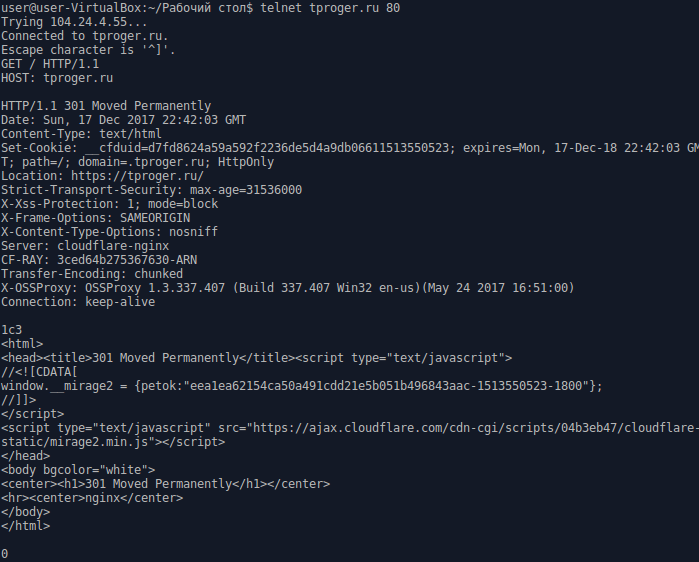
\includegraphics[scale=0.7]{http}
		\caption{Подключение к HTTP-серверу} 
		\label{pic:http} % название для ссылок внутри кода
	\end{center}
\end{figure}

\subsection{Подключение к FTP-серверу, запрос списка файлов в директории и получение файла}


C помощью команды telnet подключаемся к FTP-серверу:

\begin{lstlisting}
telnet ftp.stat.duke.edu 21
\end{lstlisting}

ftp.stat.duke.edu - ftp-сервер, к которому происходит подключение, 21 - порт.

Вводим имя пользователя и пароль. Затем необходимо перейти в пассивный режим с помощью команды pasv. С помощью цифр кодируется IP-адрес и порт для соединения. Создаем соединение к указанному IP-адресу через необходимый порт (порт высчитывается по формуле p1*256 + p2, где p1 и p2 - это два последних числа в присланном сообщении сервера). Стоит уточнить, что здесь используется одно соединение на одну команду.
С помощью команды pwd и cwd переходим по папкам рис.\ref{pic:ftp1}, пока не найдем необходимый файл. Для скачивания файла используем команду retr <имя файла>.

Файл успешно скачан (рис.\ref{pic:ftp2}).

\begin{figure}[H]
	\begin{center}
		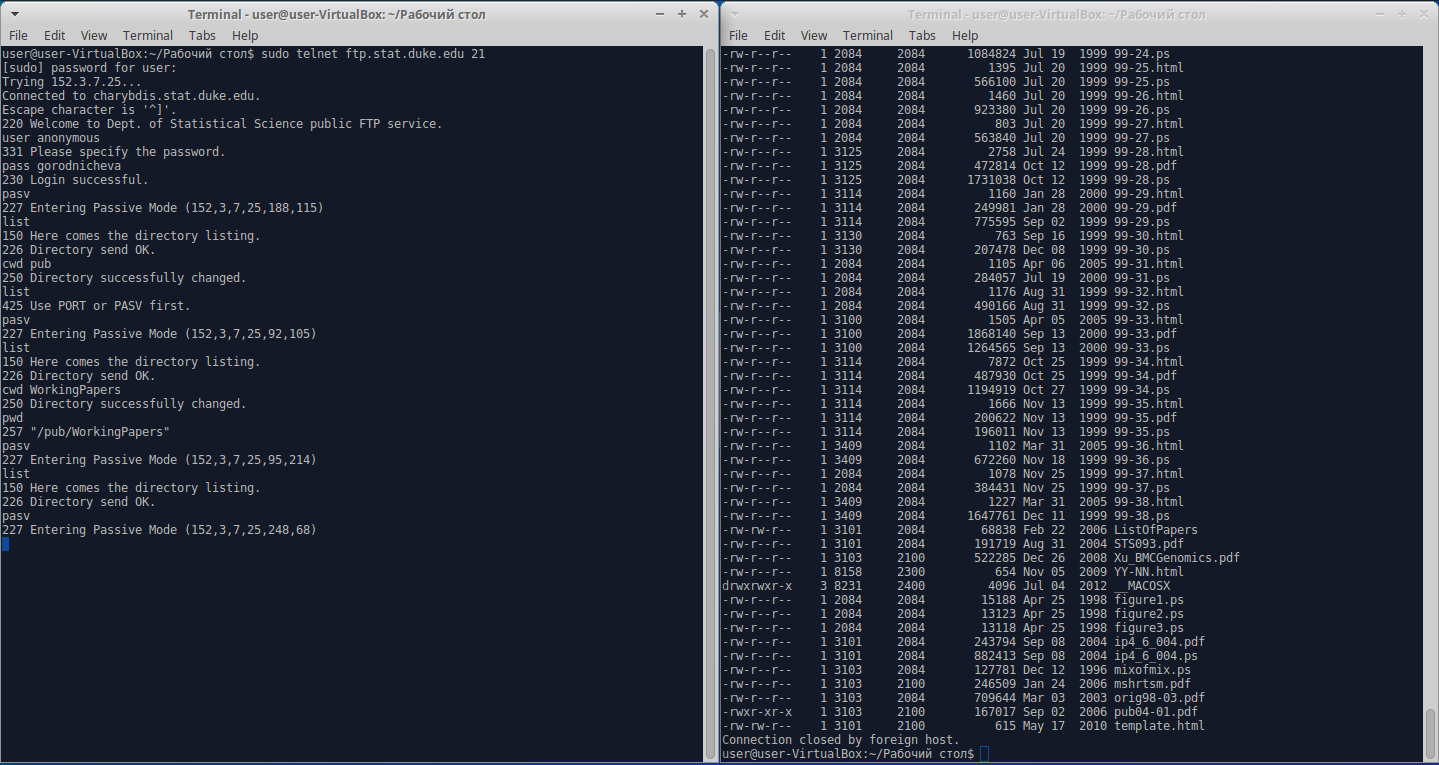
\includegraphics[scale=0.5]{ftp1}
		\caption{Подключение к FTP-серверу} 
		\label{pic:ftp1} % название для ссылок внутри кода
	\end{center}
\end{figure}

\begin{figure}[H]
	\begin{center}
		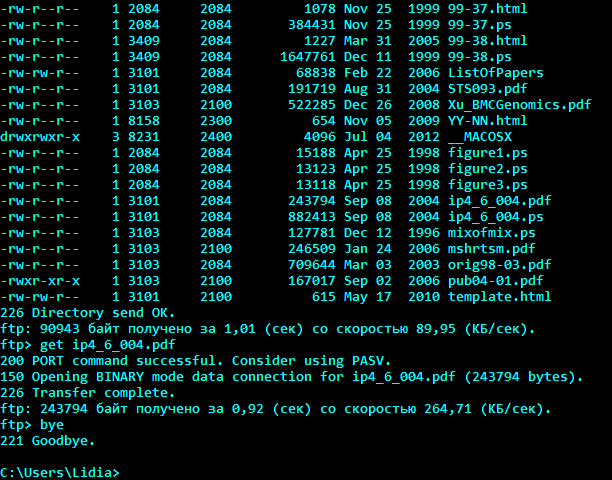
\includegraphics[scale=0.5]{ftp2}
		\caption{Скачивание файла с FTP-сервера} 
		\label{pic:ftp2} % название для ссылок внутри кода
	\end{center}
\end{figure}

\subsection{Подключение к SMTP-серверу и отправка письма}

С помощью команды, указанной ниже, подключаемся к SMTP-серверу smtp.yandex.ru (рис. \ref{pic:smtp1}):

\begin{lstlisting}
gnults-cli -p 465 smtp.yandex.ru
\end{lstlisting}

\begin{figure}[H]
	\begin{center}
		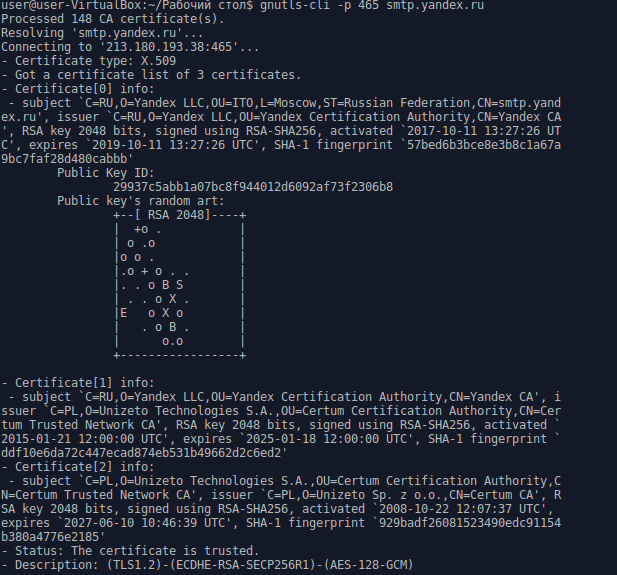
\includegraphics[scale=0.7]{smtp1}
		\caption{Подключение к SMTP-серверу} 
		\label{pic:smtp1} % название для ссылок внутри кода
	\end{center}
\end{figure}

Данная команда обеспечивает защищенное TLS-подключение. Команды telnet/nc здесь не подходят по причине их работы только с нешифрованными соединениями.  

SSL (Secure Sockets Layer) и TLS (Transport Level Security) - это криптографические протоколы, обеспечивающие защищенную передачу данных в компьютерной сети. Они активно используются при работе с электронной почтой. Соединение, защищенное протоколом TLS, обладает определенными свойствами: безопасностью, аутентификацией и целостностью. 

Затем необходимо пройти аутентификацию:

\begin{figure}[H]
	\begin{center}
		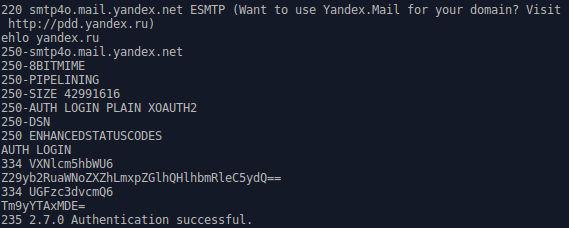
\includegraphics[scale=0.7]{smtp2}
		\caption{Аутентификация} 
		\label{pic:smtp2} % название для ссылок внутри кода
	\end{center}
\end{figure}

Для аутентификации использовался BASE64, с помощью которого были закодированы логин и пароль (рис. \ref{pic:smtp_cr}):

\begin{figure}[H]
	\begin{center}
		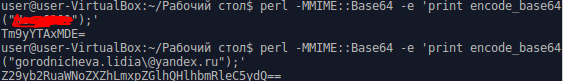
\includegraphics[scale=0.7]{smtp_cr}
		\caption{Кодирование логина и пароля} 
		\label{pic:smtp_cr} % название для ссылок внутри кода
	\end{center}
\end{figure}

 Используя команды MAIL FROM (от кого письмо), RCPT TO (кому письмо), DATA (собственно само письмо с указанием темы (Subject) и From (от кого), было отослано письмо с содержанием `Gorodnicheva Lidia'' (рис. \ref{pic:smtp3}):

\begin{figure}[H]
	\begin{center}
		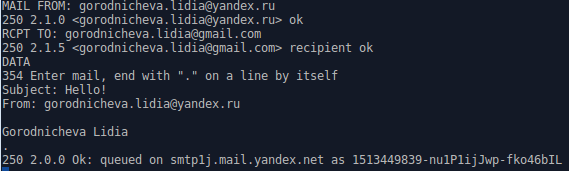
\includegraphics[scale=0.7]{smtp3}
		\caption{Посылка письма} 
		\label{pic:smtp3} % название для ссылок внутри кода
	\end{center}
\end{figure}

\subsection{Подключение к POP3-серверу, проверка почты и получение письма}

Попробуем прочитать посланное письмо с помощью протокола POP3. Для начала подключимся к POP3-серверу (рис. \ref{pic:pop1}):

\begin{figure}[H]
	\begin{center}
		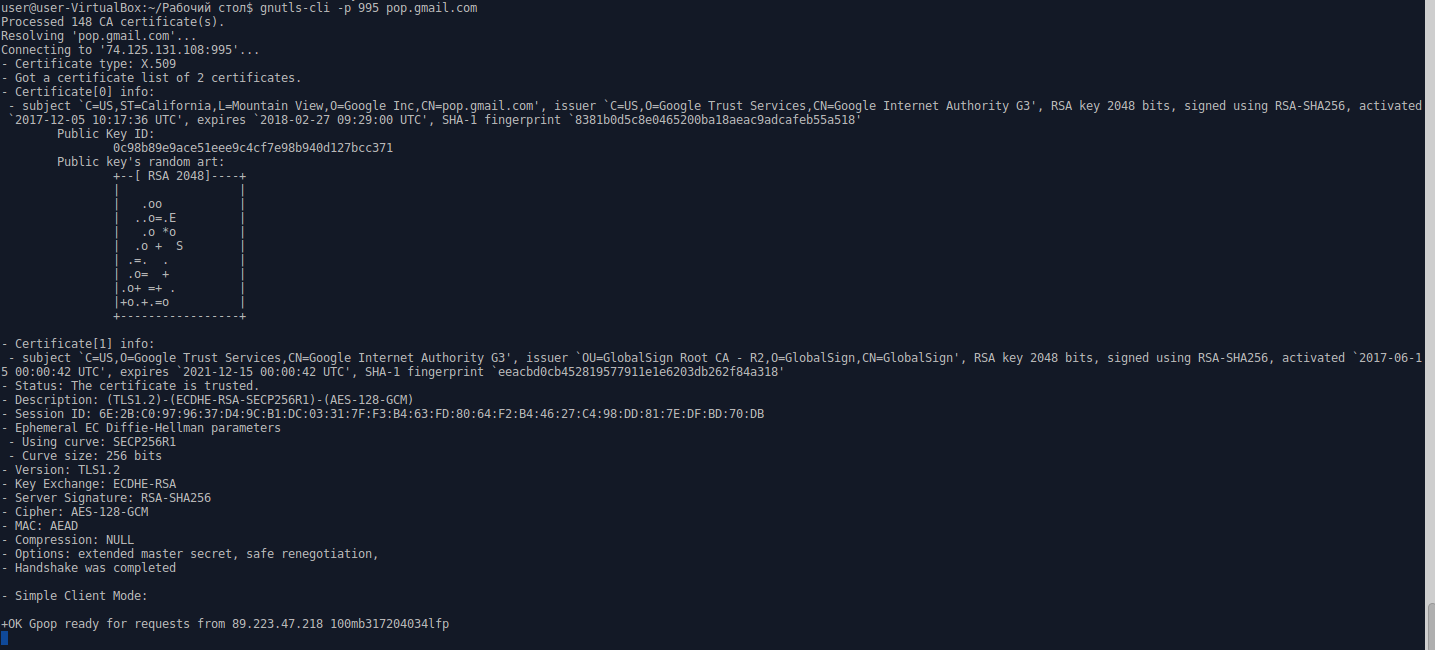
\includegraphics[scale=0.7]{pop1}
		\caption{Подключение к POP3-серверу} 
		\label{pic:pop1} % название для ссылок внутри кода
	\end{center}
\end{figure}

Затем введем логин и пароль, используя команды USER и PASS  (рис. \ref{pic:pop2}):

\begin{figure}[H]
	\begin{center}
		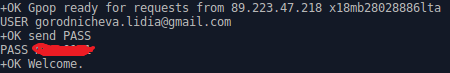
\includegraphics[scale=0.7]{pop2}
		\caption{Аутентификация} 
		\label{pic:pop2} % название для ссылок внутри кода
	\end{center}
\end{figure}

С помощью команды LIST запрошен список всем писем  (рис. \ref{pic:pop3}), а команда RETR <номер письма> вывела полученное письмо (рис. \ref{pic:pop4}):

\begin{figure}[H]
	\begin{center}
		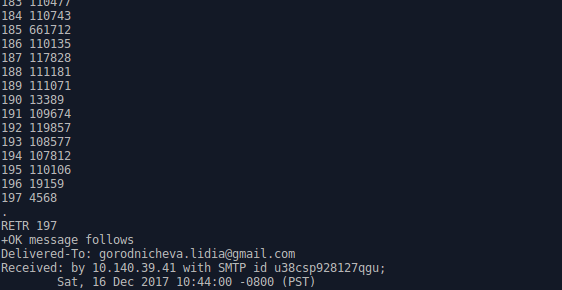
\includegraphics[scale=0.7]{pop3}
		\caption{Список писем} 
		\label{pic:pop3} % название для ссылок внутри кода
	\end{center}
\end{figure}

\begin{figure}[H]
	\begin{center}
		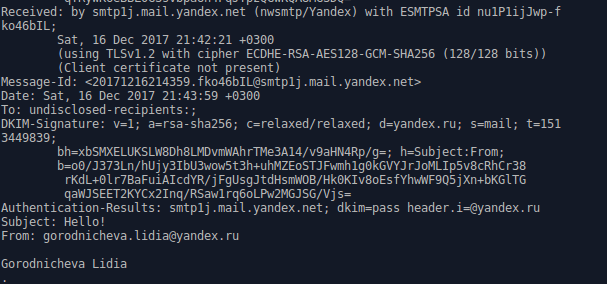
\includegraphics[scale=0.7]{pop4}
		\caption{Полученное письмо} 
		\label{pic:pop4} % название для ссылок внутри кода
	\end{center}
\end{figure}


\section{Выводы}
В данной лабораторной работе изучены принципы программирования сокетов на основе TCP и UDP. Познакомились с архитектурой разработки многопоточных сетевых приложений: использование механизма нитей и средств синхронизации. Изучение происходило через разработку простейших клиент-серверных приложений на ОС Linux и Windows, а также реализацию собственного протокола на основе TCP и UDP для индивидуального задания (а именно дистанционного тестирования). 
Чтобы не усложнять задание и не создавать отдельную базу данных для пользователей и их результатов, были созданы отдельные текстовые файлы, в которых эти пользователи хранятся. Для вопросов и вариантов ответов также есть свои файлы.
Архитектура TCP приложения была построена на основе 3 различных потоков для 3 разных видов блокирующих функций (read, accept, getline) , обеспечивая тем самым параллельную работу всей системы. Минус такой архитектуры в том, что для каждого клиента выделяется отдельный поток, что получается весьма ресурсоемко. Решить такую проблему можно, например, при помощи пула сокетов (или портов завершения, которые имеются в Windows).  
Передача сообщений по TCP тоже реализована довольно просто: мы передавали определенное количество байт с каждой посылкой, а завершали сообщение меткой.

Для передачи сообщений длиной больше, чем длина, заданная в протоколе, была создана специальная функция, которая делит сообщение на куски заданной длины и передавает их поочередно.

При разработке UDP столкнулись с тем, что соединения не создается. Чтобы сохранить простую архитектуру TCP сервера, при получении сообщения от клиента создавали новый сокет. Так было сымитировано отдельное соединение. Чтобы понимать, что все посылки доставляются верно или неверно, инкапсулировали номер посылки в сообщение. Если номер не совпадал с ожидаемым, просто выдавали ошибку. Здесь для сохранения длины посылки полную длину посылки оставили той же, однако количество байт данных в ней каждый раз меняется, в зависимости от длины номера посылки. На приеме просто отделяем номер посылки.

Также были получены навыки работы с такими прикладными протоколами, как HTTP, FTP, SMTP и POP3. Эти навыки могут оказаться полезными при разработке серьезных сетевых приложений.
Некоторые задачи данной лабораторной очень схожи с задачами, решаемыми этими протоколами. Так SMTP ожидает ответа на каждую операцию и присылает обратно код - выполнена ли операция или завершилась с какой-либо ошибкой. В нашем задании незарегистрированный и незалогиненый пользователь не может получить и пройти тест. В POP3, SMTP, а так же FTP перед тем, как выполнить какую-либо операцию, необходимо было произвести аутентификацию.

\section{Приложение}


\lstinputlisting[
	label=code:tsl,
	caption={TCP сервер на Linux},
]{tcp_server_linux.c}
\parindent=1cm

\lstinputlisting[
	label=code:tcl,
	caption={TCP клиент на Linux},
]{tcp_client_linux.c}
\parindent=1cm

\lstinputlisting[
	label=code:usw,
	caption={UDP сервер на Windows},
]{udp_server_win.c}
\parindent=1cm

\lstinputlisting[
	label=code:ucw,
	caption={UDP клиент на Windows},
]{udp_client_win.c}
\parindent=1cm


\lstinputlisting[
	label=code:mts,
	caption={Многопоточный TCP-сервер на Linux},
]{mult.c}
\parindent=1cm

\end{document}
